\documentclass[11pt, oneside]{article} 	% use "amsart" instead of "article" for AMSLaTeX format
\usepackage{geometry} 		% See geometry.pdf to learn the layout options. There are lots.
\geometry{letterpaper}  		% ... or a4paper or a5paper or ... 
\usepackage[parfill]{parskip} 		% Activate to begin paragraphs with an empty line rather than an indent
\usepackage{graphicx}				% Use pdf, png, jpg, or eps§ with pdflatex; use eps in DVI mode
								% TeX will automatically convert eps --> pdf in pdflatex		
\usepackage{amssymb}
\usepackage{amsmath}
\usepackage{authblk}
\usepackage[
backend=biber,
style=alphabetic,
]{biblatex}
\usepackage{graphicx}
\graphicspath{ {./images/} }
\usepackage{verbatim}
\usepackage{tikz} 
\usepackage{subfig}
\usepackage{hyperref}

\usepackage{syntonly}
% \syntaxonly <-- use this for checking syntax only
% \mbox {text} - keep together
% \fbox {text} - keep together and draw around

%\pagestyle{plain|headings|empty} % header and footer p.27
%SetFonts
%\include{filename}, \includeonly{filename1, filename2} , \input[fiename}

%SetFonts% 

\title{The Office DVD Problem}
\author{Dave Fetterman}
\affil{Obviously Unemployed}
\date{7/13/22}
\begin{document}
\maketitle

Screensavers have captivated [this] man since the 1990s. If watched long enough, what will the spirits of the machine tell us?

Specifically, the question of whether a bouncing rectangle will slide \emph{exactly} into the corner of the screen, for a satisfying, perfectly diametric rebound, was even addressed on \emph{The Office}
\href{https://www.youtube.com/watch?v=QOtuX0jL85Y}{(link)}.

However, though these characters reportedly watched this sleep-mode drama play out for years until payoff, we ask - under what conditions will the rectangle \emph{definitely} perfectly bounce into the screen's corner?
 
\begin{figure}
\centering
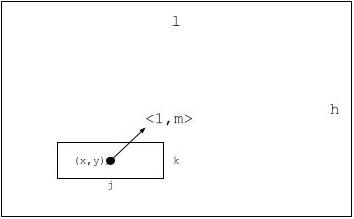
\includegraphics[scale=.5]{setup}
\caption{The Office DVD problem's most generic setup}
\end{figure}


\begin{figure}[!htb]
\centering
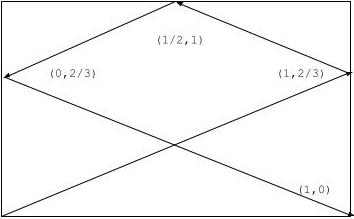
\includegraphics[scale=.5]{problem1trajectory}
 \caption{Success for $m = \frac{2}{3}, j, k = 0, h, l = 1$ (not to scale)}
\end{figure}

\subsection{Statement} 
Suppose we have a continuous screen of length $l$, height $h$, containing an axis-aligned rectangle of length $j$ and height $k$ centered at point $(x, y)$.

Suppose this rectangle is launched at direction $\langle 1, m\rangle$ \footnote {Think of this as slope $m$} and ``bounces'' according to billiard rules \footnote{Glancing off a horizontal boundary, our trajectory goes from $\langle 1, m \rangle$ to $\langle 1, -m \rangle$, with $\langle \pm 1, m \rangle$ to $\langle \mp 1, m \rangle$ for a horizontal one}.

Given $l, h, j, k, m \in \mathbb{R}$, can we tell whether the rectangle ever bounce perfectly into a corner?  

We can approach this problem from the simplest version to the most complex.

\subsection{Problem 1} 

Suppose $j = k = 0$ and $x = y = 0$. In other words, suppose we have a \emph{point} starting at the bottom left corner
 (origin). Under what conditions (i.e. choice of $m$) does this bounce into a corner?


\subsection{Problem 2} 

Suppose $j, k > 0, x = \frac{j}{2}, y = \frac{k}{2}$. In other words, suppose we have a rectangle starting at the bottom left corner. Under what conditions does this bounce into a corner?

\subsection{Problem 3} 

Suppose we have maximally open (reasonable) conditions, with $x \in [\frac{j}{2}, l - \frac{j}{2}], y \in [\frac{k}{2}, h - \frac{k}{2}]$ (that is, a $j \times k$ rectangle fitting entirely in the screen). Under what conditions does this bounce into a corner?


\subsection{Problem 4} 

Some clowns \footnote {J. H. Wang, N. H. Talbert, L. F. Waldman} have come along demanding a version of the setup respecting the discrete (pixellated) nature of digital screens.  Very well.

For each of problem 1, 2, and 3, how does the answer change if the screen comprises square pixels of length $p \in \mathbb{N}$ \footnote{If $p$ is not a whole number, this can be normalized}, where $p | j, k, h, l$, and ``meeting a corner" means a corner of the small (continuous) rectangle meets a wall within length $p$ of the corner point?


\section{Solutions}

Note: If our initial slope is zero $m = \langle 1, 0 \rangle$ or ``infinite'' ($m = \langle 0, 1 \rangle$, actually disallowed in our setup), the solution is obvious: if we're axis-aligned at the outset, we'll be in a corner shortly, otherwise we never will be.

Note also that, for the sake of simplicity, we can treat $m$ as always positive (the box going up and to the right). If not, inverting the problem ($m \rightarrow -m, y = h - y)$ will work equivalently. The box initially moving leftwards (disallowed in the problem setup) reduces to our setup by the same sort of flip.

\subsection{Problem 1 solution}

The key insight here is that though the point bounces ``within a box'' until meeting $(0,0), (0, h), (l, 0), $ or $(l, h)$ (as in Figure 2), we can instead look at the path of the point in an unconstrained space, seeing if we hit a point of the form $(a \cdot l, b \cdot h)$ with $a,b \in \mathbb{N}$.

On meeting the point $(0, \frac{2}{3})$, we can either consider what happens if we reflect ``back'' into our original box as in the left side of Figure 3, or, equivalently, if we pass ``through'' to a mirrored box on the right side of Figure 3. We quickly see that:

\begin{itemize} 
\item If the left-hand side meets a corner, the mirror-image on the right-hand side will meet a corner as well.
\item Likewise for the converse: the right meeting a corner means the left hand will as well.
\item If the left-hand side does \emph{not} meet a corner, the right-hand side cannot.
\item Likewise for the converse.
\end{itemize}

\begin{figure}[!htb]
\centering
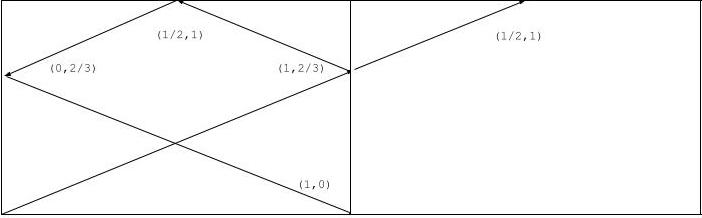
\includegraphics[scale=.5]{mirrorright}
 \caption{``Passing through'' on the right equivalent to ``bouncing back left''}
\end{figure}

Note that this applies for top-bottom just as easily as left-right (Figure 4). 

\begin{figure}[!htb]
\centering
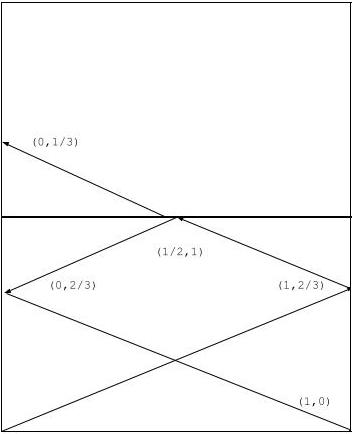
\includegraphics[scale=.5]{mirrorup}
 \caption{``Passing through'' the top equivalent to ``bouncing back down''}
\end{figure}

Therefore, composing these two, we can cast the path of the smaller rectangle as entirely ``up and to the right''. This allows us to reframe the question as: \textbf{Starting at $(0,0)$, will a line of slope $m$ reach a corner of a lattice of $l \times h$ blocks} or, equivalently, reach a point $(a \cdot l, b \cdot h)$ for some pair $a,b \in \mathbb{N}$?

\begin{figure}[!htb]
\centering
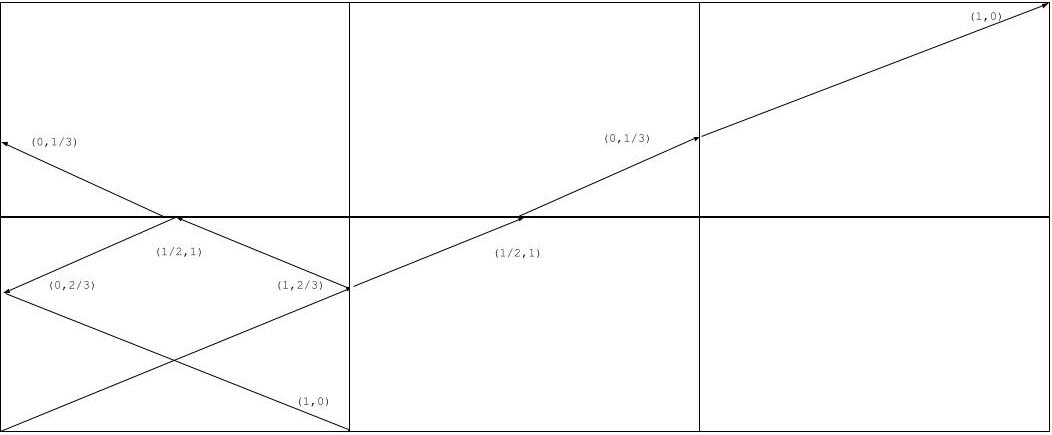
\includegraphics[scale=.4]{fullpath}
 \caption{Recasting the bouncing path as ``up and to the right'' on the l, h lattice}
\end{figure}


\begin{align}
a \cdot m \cdot l = b \cdot h \\
\frac{b}{a} = \frac{m \cdot l}{h} \\ 
\Rightarrow \frac{m \cdot l}{h} \in \mathbb{Q} 
\end{align}

We see that we reach a corner \textbf{if and only if} $\frac{m \cdot l}{h}$ is a rational number (quotient of integers).  Note that neither $m$, $h$ or $l$ can be zero from the setup, so this won't be zero or undefined.



\subsection{Problem 2 solution}

The key insight here is that instead of each ``frame'' extending from $(0, 0)$ to $(l, h)$, with the box's center ($x, y)$ constrained to the rectangle defined by $[\frac{j}{2}, l - \frac{j}{2}], \times [\frac{k}{2}, h - \frac{k}{2}]$, we can instead treat the \emph{center} of that $[\frac{j}{2}, l - \frac{j}{2}], \times [\frac{k}{2}, h - \frac{k}{2}]$ box as a point like in problem 1. 

It is then clear that we can use problem 1's main insight to the center point as opposed to the small rectangle: that the small rectangle, say, $\frac{j}{2}$ left of the right border of one frame will take an trajectory eqjuivalent to that of a rectangle $\frac{j}{2}$ right of the left border of the adjoining right frame.

So, restate the problem as $j, k = 0; l \rightarrow l - j; h \rightarrow h - k;  x \rightarrow x - \frac{j}{2}; y \rightarrow y - \frac{k}{2}$ and solve as in problem 1.

\begin{figure}[!htb]
\centering
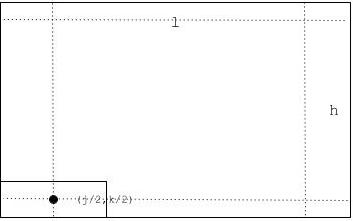
\includegraphics[scale=.4]{problem2}
\caption{The center of a $j \times k$ rectangle is a point bouncing in the $(l - j) \times (h - k)$ box}
\end{figure}

\subsection{Problem 3 solution}

Here, we're looking at the set of solutions where $(x, y) \neq (0, 0)$.

For simplicity, we'll consider only a zero-dimensional rectangle ($j = k = 0$) here; otherwise, it can be reduced as in the solution to problem 2 before coming back here.

It's clear that there are many non-solutions here. Consider, on a grid $h = l = 1$, starting at point $(\frac{1}{2}, 0)$ with a slope $m = 1$. The point will clearly bounce around between $(1, \frac{1}{2}), (\frac{1}{2}, 1), (0, \frac{1}{2})$ and $ (\frac{1}{2}, 0)$ forever without meeting a corner (Figure 7).

\begin{figure}[!htb]
\centering
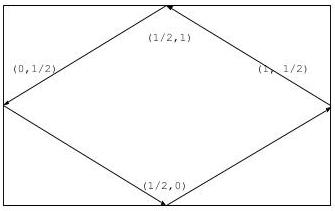
\includegraphics[scale=.4]{bounceforever}
\caption{$(x, y) = (\frac{1}{2}, 0), m = 1$ bounces forever}
\end{figure}

First, find the intercept with the next x boundary as in Figure 8.

\begin{figure}[!htb]
\centering
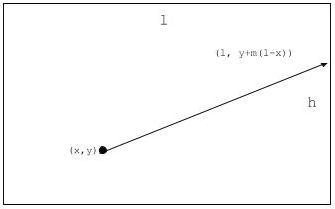
\includegraphics[scale=.4]{intercept}
\caption{Finding the intercept $y^* = y + m(l-x)$}
\end{figure}

If we're going to end in a corner, then adding this intercept $y^*$ this to a series of $a$ `runs' of length $l$ should meet at a lattice point of $b$ `rises' of height $h$, according to slope $m$. Note that $y^*$ may be greater than $h$ (so it could be many ``squares up''), and also note that if $y^* = 0$, then we're already found our corner. 

Given all of these quantities $y^*, m, h, l$, we're looking to discover nonnegative integers $a$ and $b$ that allow us to solve this equation:

\begin{align}
y^* + a\cdot m \cdot l = b \cdot h, a, b \in \mathbb{N} \\ 
y^* = b \cdot h -  a\cdot m \cdot l \\
1 = b \cdot \frac{h}{y^*} -  a\cdot \frac{m \cdot l}{y^*} 
\end{align}

There are four (not entirely separate) cases here:

\begin{itemize}
\item $\frac{h}{y^*}, \frac{m \cdot l}{y^*}$ are both integers. In this case, we can use Euler's algorithm to find the greatest common denominator of $\frac{h}{y^*}, \frac{m \cdot l}{y^*}$, as well as $b$, $a$. If that GCD equals one, the algorithm will give us $b$ and $a$. Otherwise, there is no solution (we never hit a corner).
\item $\frac{h}{y^*}, \frac{m \cdot l}{y^*}$ are rational but there is at least one non-integer among them. In this case, multiply out the denominators by the necessary factor $d$ to make them integers, and reduce to the first case looking for GCD $d$. If our GCD is $d$ or divides $d$, we will hit a corner, otherwise we will bounce infinitely. Note that Figure 7's scenario ($y^* = \frac{3}{2}, m = h = l = 1$) reduces to $1 = b \cdot \frac{2}{3} - a  \cdot \frac{2}{3} \Rightarrow 3 = 2a-2b$, which has no integer solution pair.
\item Exactly one of $\frac{h}{y^*}, \frac{m \cdot l}{y^*}$ is irrational. Then there is clearly no solution without $a$ or $b$ equaling zero (which we've eliminated).
\item Both $\frac{h}{y^*}, \frac{m \cdot l}{y^*}$ are irrational. This reduces to:
\begin{align}
\frac{y^*}{h} = b - a\frac{m \cdot l}{h} \\
-\frac{y^*}{h} = a\frac{m \cdot l}{h} \mod 1 
\end{align}
Though we look close to a solution, this rearranging hasn't gotten us much farther since we can't multiply by $\frac{h}{m \cdot l}$ while retaining modulus 1. For example, try corner-bouncer $y^* = 1+\sqrt{2}, l = 1, h = \frac{1}{2} + \sqrt{2}, m = \sqrt{2}$, yielding $a = 1, b = 2$; equation (8) is satisfied but multiplying by $\frac{h}{m \cdot l}$ doesn't work. The best we can hope for is that $-y^*$ and $m \cdot l$ have an obvious relationship.

\end{itemize}

As an aside, the likelihood that a randomly chosen set of reals $y^*, m, h, l$ will produce a corner bump is zero.  To see this, let's take a set $h, l, m$ and replace $m \rightarrow m \frac{l}{h}$ so we can consider $h, l = 1$. 

Let's say our intercept happens one block to the right. This fixes our $y^*$ to a single, determined value. Same with two blocks, three, etc. Assuming there is an intercept somewhere down the line, there are a countable number of $y^*$ selections which will make this system work, one for each integer greater than zero. However there are certainly an \emph{uncountable} number of $y^*$ selections with $y^* \in (0, 1)$!


\subsection{Problem 4 solutions}

First, note that any successful bounce trajectory for the continuous case implies a successful pixellated trajectory as well (meeting the corner perfectly is stricter than meeting approximately).

To define the success conditions, we're looking for instances of $a \in \mathbb{N}$ where $y^* + a \cdot m \cdot l \mod h > h - \frac{h}{p} $ or $y^* + a \cdot m \cdot l \mod h  <= h/p$. \footnote {Let's arbitrarily assume we round ``left and down'' when pixel mapping on exact borders}.

With the main (``up and to the right'') intuition from Solution 1 in hand, consider that as point travels right, it will meet right-hand walls (where $x = a \cdot l, l \in \mathbb{N}$) with various heights within the $[l, h]$ box.  The first such height will be at $y^*$ as defined in solution 1, the second at $y^* + 1 \cdot m \cdot l \mod h$, then at $y^* + 2 \cdot m \cdot l \mod h$, $y^* + 3 \cdot m \cdot l \mod h$, etc. on to infinity (Figure 9).



\begin{figure}[!htb]
\centering
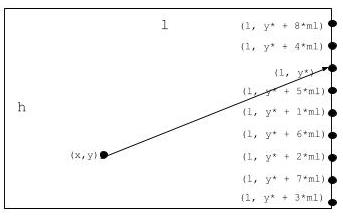
\includegraphics[scale=.4]{iteratedintercepts}
\caption{Iterated right-wall intercepts modulo h}
\end{figure}



\subsubsection{Problem 4.1 Solution}

From problem 1, if $\frac{m \cdot l}{h}$ is rational, we will meet a corner.  Restated, if we hit a corner, there are $a, b \in \mathbb{N}$ 
such that  
\begin{align}
\frac{b}{a} = \frac{m \cdot l}{h} \\
 \Rightarrow a \cdot ml = b \cdot h \\ 
  \Rightarrow a \cdot ml = 0 \mod h  
\end{align}

This means that our right wall is divided into some number $a$ \footnote{Technically, some number dividing $a$} of equal-sized steps (modulo $h$) before meeting a $0\mod h$ case, as above in figure 9.  

However, if $\frac{m \cdot l}{h}$ is \emph{ir}rational, we will fill up the line with a countably infinite number of evenly spaced points modulo $h$.  One of them will necessarily land within $p$ of a corner. 

So in a pixellated universe, for the setup of problem 1, we will \emph{always} meet a corner.



\subsubsection{Problem 4.2 Solution}

As far as I can tell, nothing changes about this when reframed in the pixellated universe.  We're still operating under continuous dimensions, but only changing the conditions under which a corner is reached.

\subsubsection{Problem 4.3 Solution}

In our pixellated case, we necessarily suppose that $l, h \in \mathbb{N}$.  By solution 4.1, if $\frac{ml}{h}$ is irrational, we will hit a corner. Therefore, we need only consider when $m$ is rational, expressed as some $m = \frac{v}{w}$ with $ v, w \in \mathbb{N}$.

Then we're looking $| y^* + aml - bh | < p \Rightarrow |y^*w+ amlw - bhw| < pw$. 

Reducing this to a set of integer equations, this means that hitting a right wall within the pixel boundary means we satisfy at least one of:

\begin{itemize}
\item $\lfloor y^*w \rfloor + amlw = 0 \mod hw$
\item $\lfloor y^*w \rfloor + amlw = 1 \mod hw$
\item ...
\item $\lfloor y^*w \rfloor + amlw = pw-1 \mod hw$
\item $\lceil y^*w \rceil + amlw = 0 \mod hw$
\item $\lceil y^*w \rceil + amlw = -1 \mod hw$
\item ...
\item $\lceil y^*w \rceil + aml = -pw+1 \mod hw$
\end{itemize}


This is, again, somewhat unsatisfying.  

There are two shortcuts.

Take the lowest $a$ that satisfies equation (11) above.  This lets us know how many contact intervals the right wall is divided into, their width modulo $h$ being $\frac{h}{a}$. If $\frac{h}{a} <= 2p$, one of these contact points falls within one $p$ above or below a corner, a ``hit'' by our definition.

Otherwise, we have a small number of contact points, and we can simply simulate (play out) the bounces, which may be fewer that $2pw$ equations to check above.

Note also that we need to check the top edge of the corner as well, or $b \cdot \frac{h}{m} = 0 \mod l$. Consider $h = 10, l = 10, m = 10, p = 1, (x, y) = (0, 5)$.  So, by the same logic, if $\frac{l}{b} <= 2p$, we also find a solution.  The above logic should be repeated with $| x^* + a\frac{h}{m} - bl | < p$ in case we're in one of these ``vertically bouncy'' scenarios.










\end{document}
